
%-----------------------------
%	PACKAGES
%-----------------------------

\documentclass[paper=letter, fontsize=12pt]{article} % Letter paper and 11pt font size

\usepackage[english]{babel} % English language/hyphenation
\usepackage{amsmath,amsfonts,amsthm} % Math packages
\usepackage{setspace}
\usepackage{sectsty} % Allows customizing section commands
\usepackage{pdfpages}
\usepackage{graphicx}

\usepackage{fancyhdr} % Custom headers and footers
\pagestyle{fancyplain} % Makes all pages in the document conform to the custom headers and footers
\fancyhead{} % No page header - if you want one, create it in the same way as the footers below
\fancyfoot[L]{} % Empty left footer
\fancyfoot[C]{} % Empty center footer
\fancyfoot[R]{\thepage} % Page numbering for right footer
\renewcommand{\headrulewidth}{0pt} % Remove header underlines
\renewcommand{\footrulewidth}{0pt} % Remove footer underlines
\setlength{\headheight}{0pt} % Customize the height of the header

%margin
\addtolength{\textwidth}{1.5in}
\addtolength{\textheight}{1.50in}
\addtolength{\hoffset}{-0.75in}
\addtolength{\voffset}{-0.75in}


%-----------------------------
%	TITLE SECTION
%-----------------------------

\newcommand{\horrule}[1]{\rule{\linewidth}{#1}} % Create horizontal rule command with 1 argument of height

\title{
\normalfont \normalsize 
\horrule{2pt} \\
\LARGE Nearest Neighbor Search Data Structure \\ [-10 pt] %title
\horrule{1pt} \\
}

\author{
	\small
	\begin{tabular}{*{3}{c}}
		\textbf{Sanjoy Dasgupta} & \textbf{Zhen Zhai} & \textbf{Eugene Che} \\
		Department of Computer Science & Department of Computer Science & Department of Computer Science  \\
		University of California, San Diego & University of California, San Diego & University of California, San Diego \\
		dasgupta@cs.ucsd.edu & zzhai@ucsd.edu & eche@ucsd.edu \\
	\end{tabular}
}
 
\date{}

\begin{document}

\maketitle

\begin{abstract}
Nearest-neighbor(NN) search is boardly used within all different fields of study to gain information on new data from training data set. For NN search, the more complex the training data set is the more accurate the result will be. However, doing NN search on complex and large training data sets is time consuming. Therefore, improving the speed and acuracy of nearest-neighbor search becomes essential. We look at different data structures for NN search and compare the results on varied data sets. We focus on data structures including KD tree and PCA tree. We also look at KD spill tree, KD virtual spill tree, and PCA spill tree to explore about the technique of spilling and virtual spilling. We conclude that spilling and virtual spilling improve the performance of the data structures.
\end{abstract}

\section{Introduction}
Gaining information of an input query by looking for the most similar match from the training set is referred as nearest neighbor(NN) search. We are given a data set $\mathbf S$ that contains a set of points $\{ s_1, s_2, s_3, ... , s_n\}$ and an input query $q$, and we are looking for the nearest neighbor $s_i$ of $q$ in $\mathbf S$ such that $s_i$ can provide valuable information about input query $q$.\\
\hspace*{2em} A lot of machine learning algorithms spend a big amount of time on nearest neighbor search. The reason that NN search is time consuming is that the training set could very well be represented by high dimentional vectors. In fact, the accuracy of the NN search result is proportional with the complexity of the training set. Therefore, speeding up NN search can lead to tremoudous improvment to many applications of not only machine learning but also data analysis, bio-informatics, signal processing, etc.\\
\hspace*{2em} There has been a large number of research devoting to speed up the performance of NN search. In this paper, we evaluate two most promising data structures, KD tree and PCA tree. We conclude that PCA tree has better performance than KD tree.\\
\hspace*{2em} We also experiment the technique of spilling by looking at KD spill tree vs. KD tree and PCA spill tree vs. PCA tree. We observe that spilling gives a better result.\\
\hspace*{2em} We finally experiment the technique of virtual spilling by looking at KD virtual spill tree. We compare it with KD spill tree and conclude that virtual spilling improve the performance of spilling.\\
\hspace*{2em} We apply these data structures on five different data sets from different area of study including computer vision, human relationship... We focus on the accuracy of NN search using these data structures and make sure it generally apply to all different kinds of data sets. In conclusion, we observe the following: PCA tree has a better performance comparing to KD tree, spilling improve the performance, and virtual spilling improve the accuracy slightly more than spilling.



\section{KD tree vs. PCA tree}
We focus our study on binary space partitioning(BSP) trees, one of the most promising data structure for NN search. We first look at k-dimentional(KD) trees. Then we study principle component analysis(PCA) tree, in which we preprocess the data using PCA(Pearson, 1901) before partitioning the space.


\subsection{KD trees}
KD tree is a BSP tree that partition data points into a k dimentional binary tree(Bentley, 1975). Starting from the root of the tree, a cooridnate with biggest variance is chosen. The data points $\mathbf S$ from root are split at the median of the coordinate into two children of the root. Recursively apply the process on the children until the leaf of the tree contain at most $\mathbf n_0$ data points.\\
\hspace*{2em} Given KD tree $T$ and query $q$, simply trace $q$ down the tree and find the leaf $l$ it falls in. Return all the possible nearest neighbors within leaf $l$. Then do distance calculation for each of the data point in leaf and return the point that lies closest to query $q$.
\\~\\
Pseudocode:\\
\hspace*{1em} \textbf{function BuildTree(S)}\\
\hspace*{2em} If $|S| < n_0:$\\
\hspace*{3em} return $S$\\
\hspace*{2em} Choose the coordinate $c$ with max variance\\
\hspace*{2em} Split $S$ into $L$ and $R$:\\
\hspace*{3em} $m = median \{ x_c: x \in S\}$\\
\hspace*{3em} $L = \{ x \in S: x_c \leq m\}$\\
\hspace*{3em} $R = \{ x \in S: x_c > m\}$\\
\hspace*{2em} $L = BuildTree(L)$\\
\hspace*{2em} $R = BuildTree(R)$\\
\hspace*{2em} return ($c, m, L, R$)\\~\\
\hspace*{1em} \textbf{function SearchTree(T)}\\
\hspace*{2em} If $T$ is leaf\\
\hspace*{3em} return $NN(q, T)$\\
\hspace*{2em} If $q[c] < m$\\
\hspace*{3em} return $SearchTree(L)$\\
\hspace*{2em} Else\\
\hspace*{3em} return $SearchTree(R)$\\~\\
\hspace*{1em} \textbf{function NN(q, S)}\\
\hspace*{2em} brute-force search closest data $d$ of $q$\\
\hspace*{2em} return $d$
\\~\\
\hspace*{2em} The problem with KD tree is that the true nearest neighbor $n$ of query $q$ could be in a leaf that is different from the leaf $q$ falls in. This could happen easily when $q$ and $n$ are both located close to the boundary of the tree (Figure 1). Therefore, the error rate could be very high.


\subsection{PCA tree}
PCA tree is also a BSP tree which partition data after a process of PCA on the data points. From the root of the tree, we do PCA and find the first principle component $\mathbf{v}$. We then reduce the dimension of the data by mapping all the data points onto $\mathbf{v}$ which gives us a one dimensional data set $s$. The original data points from root are partition using the corresponding data in $s$ and split at the median of $s$.\\
Similar to KD tree, searching NN of a query $q$ can be done by tracing $q$ down the tree.
\\~\\
Pseudocode:\\
\hspace*{1em} \textbf{function BuildTree(S)}\\
\hspace*{2em} If $|S| < n_0$\\
\hspace*{3em} return $S$\\
\hspace*{2em} Run PCA and find the first principal component $\mathbf{v} \in \mathbb{R}^d$\\
\hspace*{2em} $m$ = median $\{x \cdot c: x\in S\}$\\
\hspace*{2em} Split $S$ into $L$ and $R$:\\
\hspace*{3em} $L = \{x: x\cdot c \leq m\}$\\
\hspace*{3em} $R = \{x: x\cdot c > m\}$\\
\hspace*{2em} $L = BuildTree(L, n)$\\
\hspace*{2em} $R = BuildTree(R, n)$\\
\hspace*{2em} return ($c, m, L, R$)\\~\\
\hspace*{1em} \textbf{function SearchTree(T)}\\
\hspace*{2em} If $T$ is leaf\\
\hspace*{3em} return $NN(q, T)$\\
\hspace*{2em} $q_c = q \cdot c$\\
\hspace*{2em} If $q_c < m$\\
\hspace*{3em} return $SearchTree(L)$\\
\hspace*{2em} Else\\
\hspace*{3em} return $SearchTree(R)$
\\~\\
PCA tree has the similar problem with KD tree that $q$ could falls into different leaf. However, because of the PCA process, the probability of $q$ falling into different leaf is smaller. (EXPLAIN HERE)


\subsection{Experimental results}

We examine the performance of KD tree and PCA tree with five different data sets. (WRITE ABOUT EXPERIMENT DATA SET HERE)

\begin{figure}[h]
   \centering
   \begin{tabular}{c c}
   	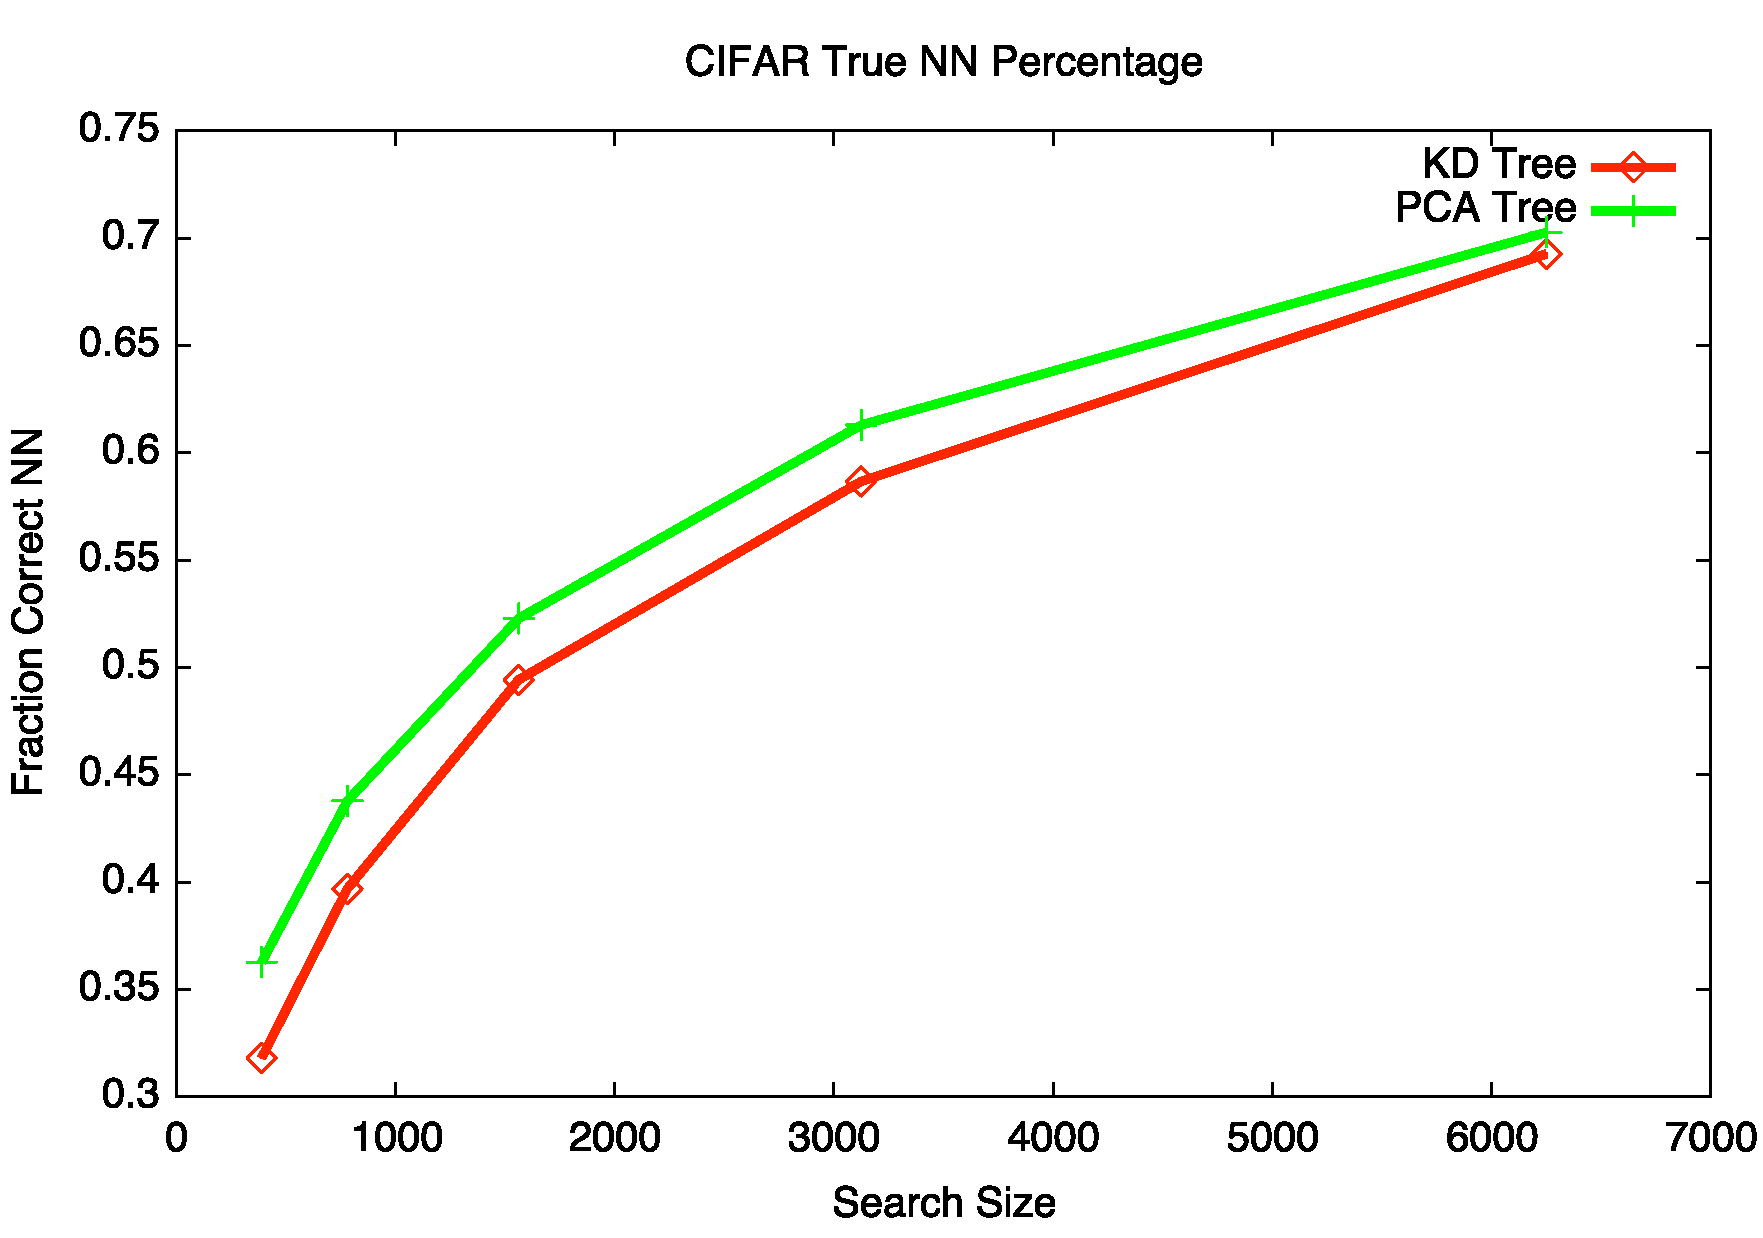
\includegraphics[width=.5\textwidth]{kd_vs_pca.pdf}
   \end{tabular}
\end{figure}

\section{Spilling or not}
We explore the technique of spilling on both KD tree and PCA tree.  Experiment supports that spilling improve the accuracy of NN search.

\subsection{Spilling}
Spilling is a technique used when building a tree with spill factor $\alpha$. Starting from the root of the tree, a cooridnate $c$ is chosen. The data points $\mathbf S$ from root are split at the median of the coordinate into two children of the root. Some data points which fall into the range of the spilling factor $\alpha$ are placed in both of the children. Recursively apply the process on the children until the leaf of the tree contain at most $\mathbf n$ data points. The search function is same as previous stated.\\
\\~\\
Pseudocode of KD Spill Tree:\\
\hspace*{1em} \textbf{function BuildTree(S)}\\
\hspace*{2em} If $|S| < n_0$\\
\hspace*{3em} return $S$\\
\hspace*{2em} Choose the coordinate $c$ with max variance\\
\hspace*{2em} Split $S$ into $L$ and $R$:\\
\hspace*{3em} $m = median \{ x_c: x \in S\}$\\
\hspace*{3em} $L = \{ x \in S: x_c \leq m\}$\\
\hspace*{3em} $R = \{ x \in S: x_c > m\}$\\
\hspace*{2em} Find spill range ($r_1$, $r_2$):\\
\hspace*{3em} $r_1 = (0.5-\alpha)quantile  \{ x_1: x \in S\}$\\
\hspace*{3em} $r_2 = (0.5+\alpha)quantile \{ x_2: x \in S\}$\\
\hspace*{2em} If $\{d \in S:  r_1 < d < r_2\}$:\\
\hspace*{3em} $L.add(d)$\\
\hspace*{3em} $R.add(d)$\\
\hspace*{2em} $LeftTree = BuildTree(L)$\\
\hspace*{2em} $RightTree = BuildTree(R)$\\
\hspace*{2em} return $(c,m)$
\\~\\
\hspace*{2em} We try to increase the accuracy by examing through the data which lie close to the boundary. The distance from the boundary is determined by the spill factor $\alpha$. The bigger the $\alpha$ the more the data we need to examine. To maintain the efficiency of KD tree algorithm, we keep the value of $\alpha$ small and we compare performance of different values of $\alpha$.


\subsection{Experimental results}
In the following experiments, we apply two different values of $\alpha$: 0.05 and 0.1. We compare the performance of KD tree vs. KD spill tree and PCA tree vs. PCA spill tree to evaluate the improvement of spilling.
\begin{figure}[h]
   \centering
   \begin{tabular}{c c}
   	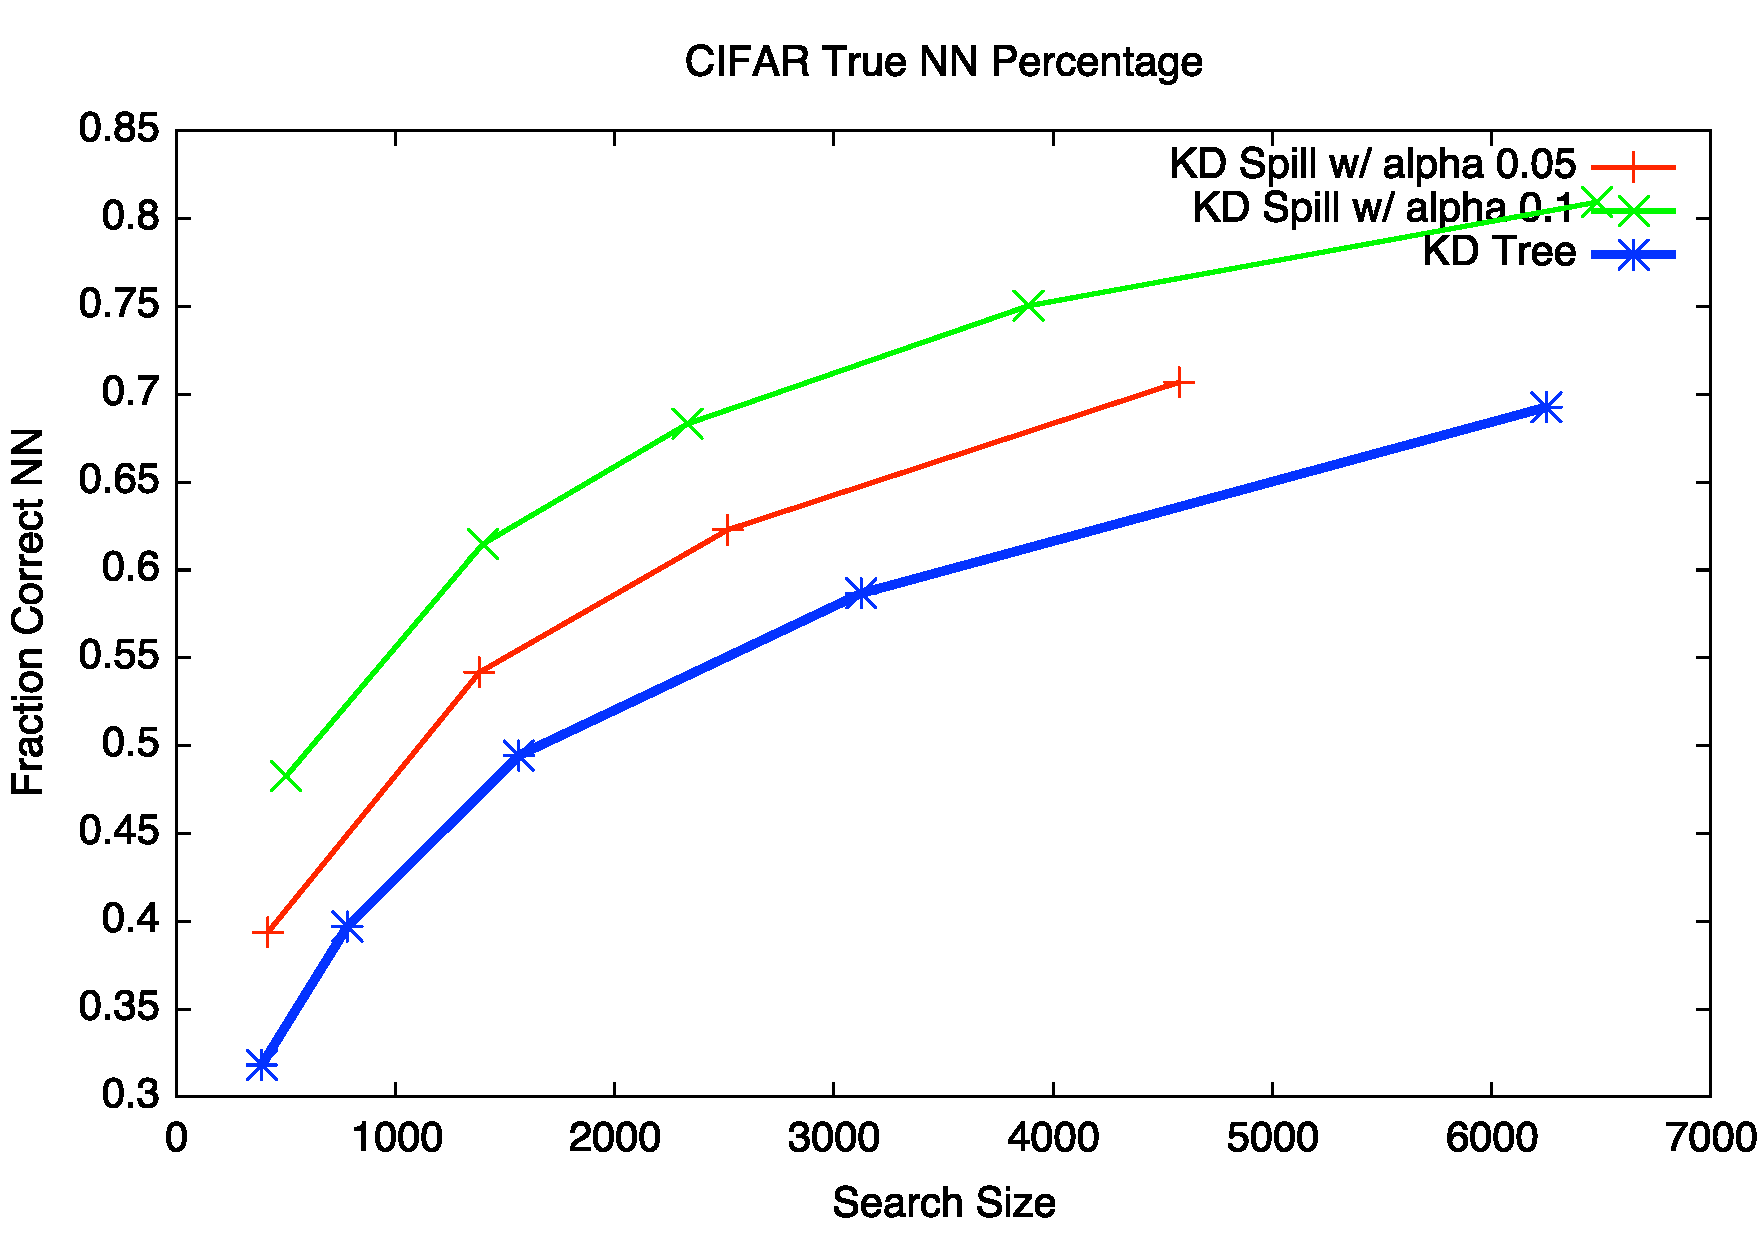
\includegraphics[width=.5\textwidth]{kd_vs_spill.pdf} &
   	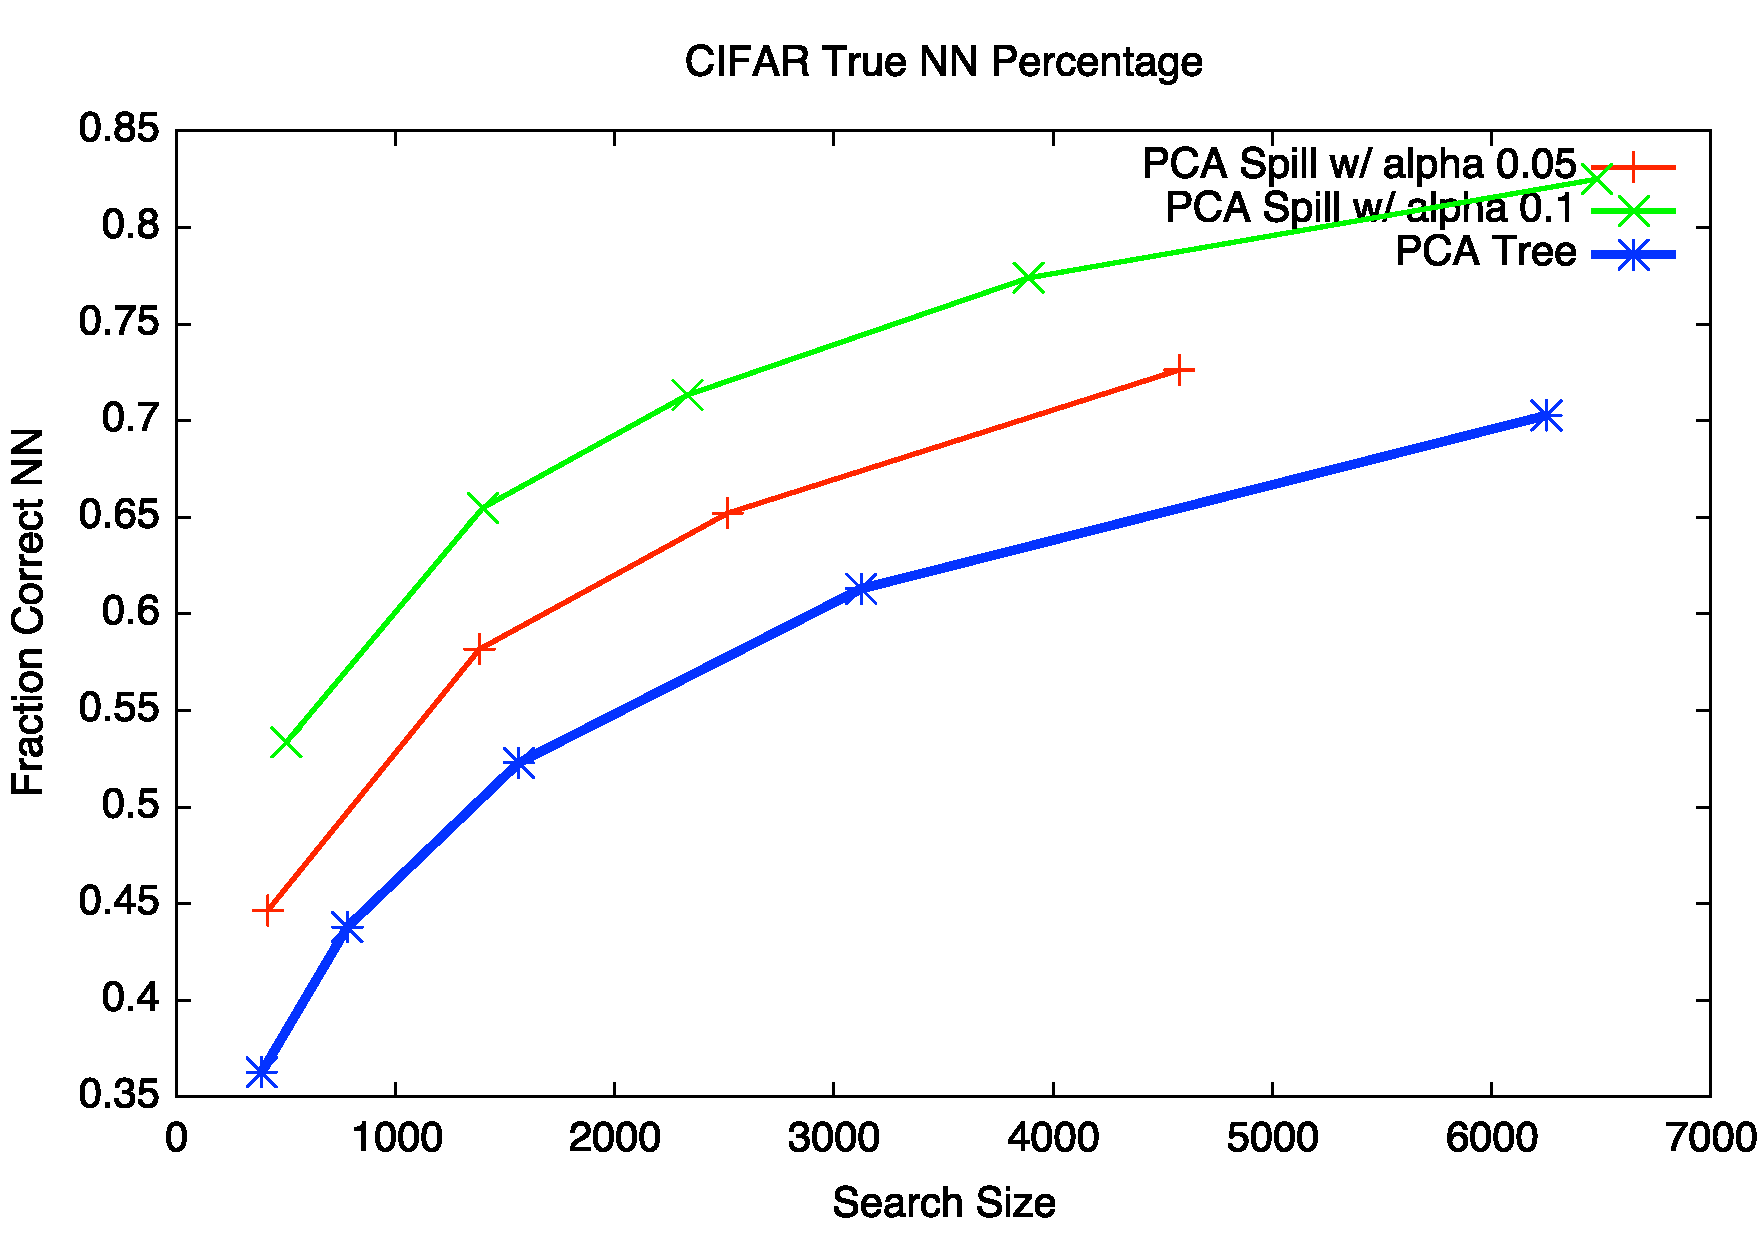
\includegraphics[width=.5\textwidth]{pca_vs_spill.pdf}
   \end{tabular}
\end{figure}


\section{Virtual spill tree vs. spill tree}
We now look at a revised spilling technique, virtual spilling. We compare the performance of KD virtual spill tree with KD spill tree.

\subsection{Virtual spill tree}
Virtual spilling is a technique used in the searching process of the tree. Given KD tree $T$ and query $q$, trace $q$ down the tree and find the leaf(ves) $l$ it falls in. If $q$ fall into the range of the spill factor $\alpha$ of a node, trace both of the children of the node. Return all the possible nearest neighbors $nn$ within the leaf(ves) $l$. Then do distance calculation for each of the data point in each leaf and return the point that lies closest to query $q$ among all leaves.
\\~\\
Pseudocode:\\
\hspace*{1em} \textbf{function SearchTree(T)}\\
\hspace*{2em} If $T$ is leaf\\
\hspace*{3em} return $NN(q, T)$\\
\hspace*{2em} Find spill range ($r_1$, $r_2$):\\
\hspace*{3em} $r_1 = (0.5-\alpha)quantile  \{ x_1: x \in S\}$\\
\hspace*{3em} $r_2 = (0.5+\alpha)quantile \{ x_2: x \in S\}$\\
\hspace*{2em} If $r_1 < q[c] < r_2$\\
\hspace*{3em} $nn.add(SearchTree(L))$\\
\hspace*{3em} $nn.add(SearchTree(R))$\\
\hspace*{2em} Else if $q[c] < m$\\
\hspace*{3em} $nn.add(SearchTree(L))$\\
\hspace*{2em} Else if $q[c] > m$\\
\hspace*{3em} $nn.add(SearchTree(R))$\\
\hspace*{2em} return $NN(q,nn)$
\\~\\
\hspace*{2em} Virtual spill tree is also aim at increasing the accuracy by examing datas lie near boundary. However, unlike spill tree, where $\alpha$ determine the range of examination, virtual spill tree examine the adjacent leaves if the query falls into the spilling range which is determined by $\alpha$.


\subsection{Experimental results}
Similar to the experiment on spill tree, we focus on $\alpha$ being 0.05 and 0.1. We see that the accuracy is increased by using the virtual spilling technique on KD tree.
\begin{figure}[h]
   \centering
   \begin{tabular}{c c}
   	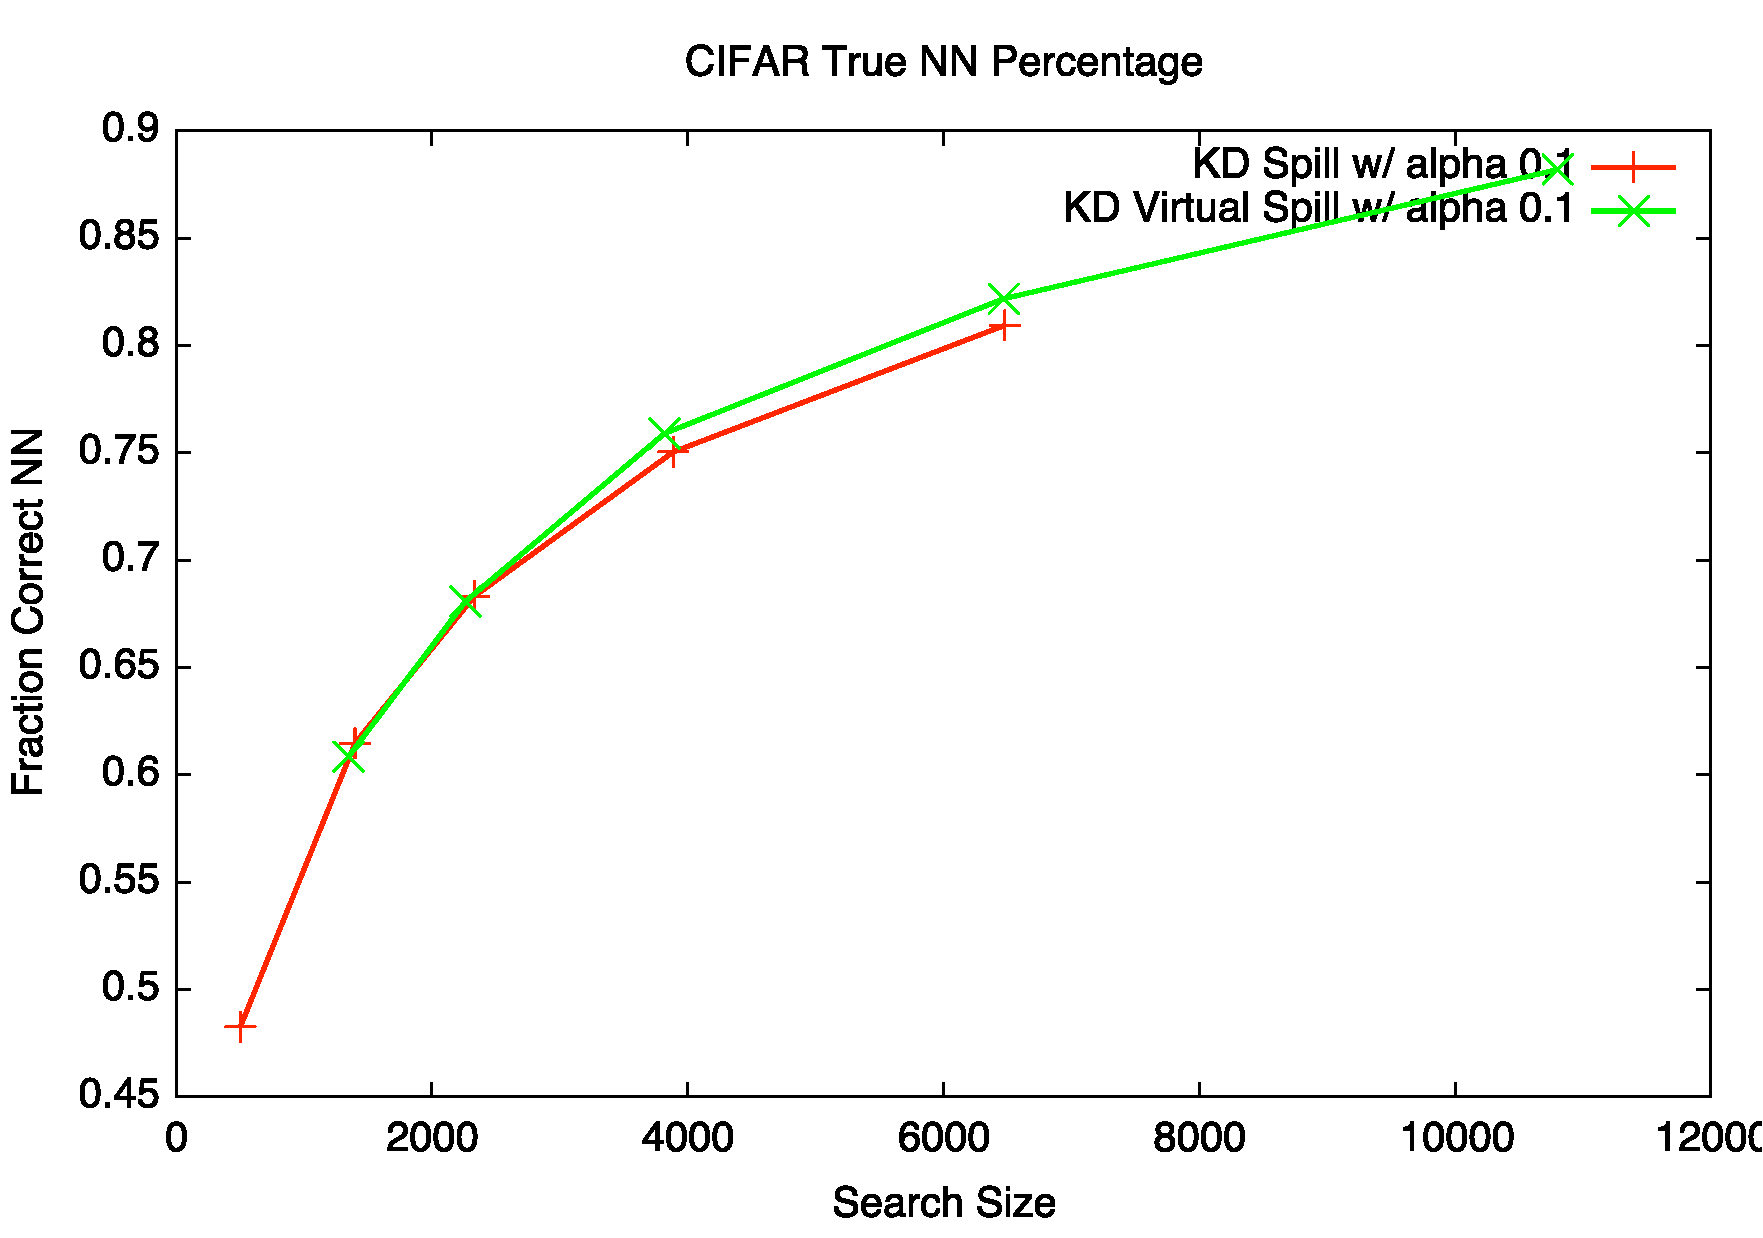
\includegraphics[width=.5\textwidth]{kd_vspill_vs_kd_spill_point1.pdf} &
   	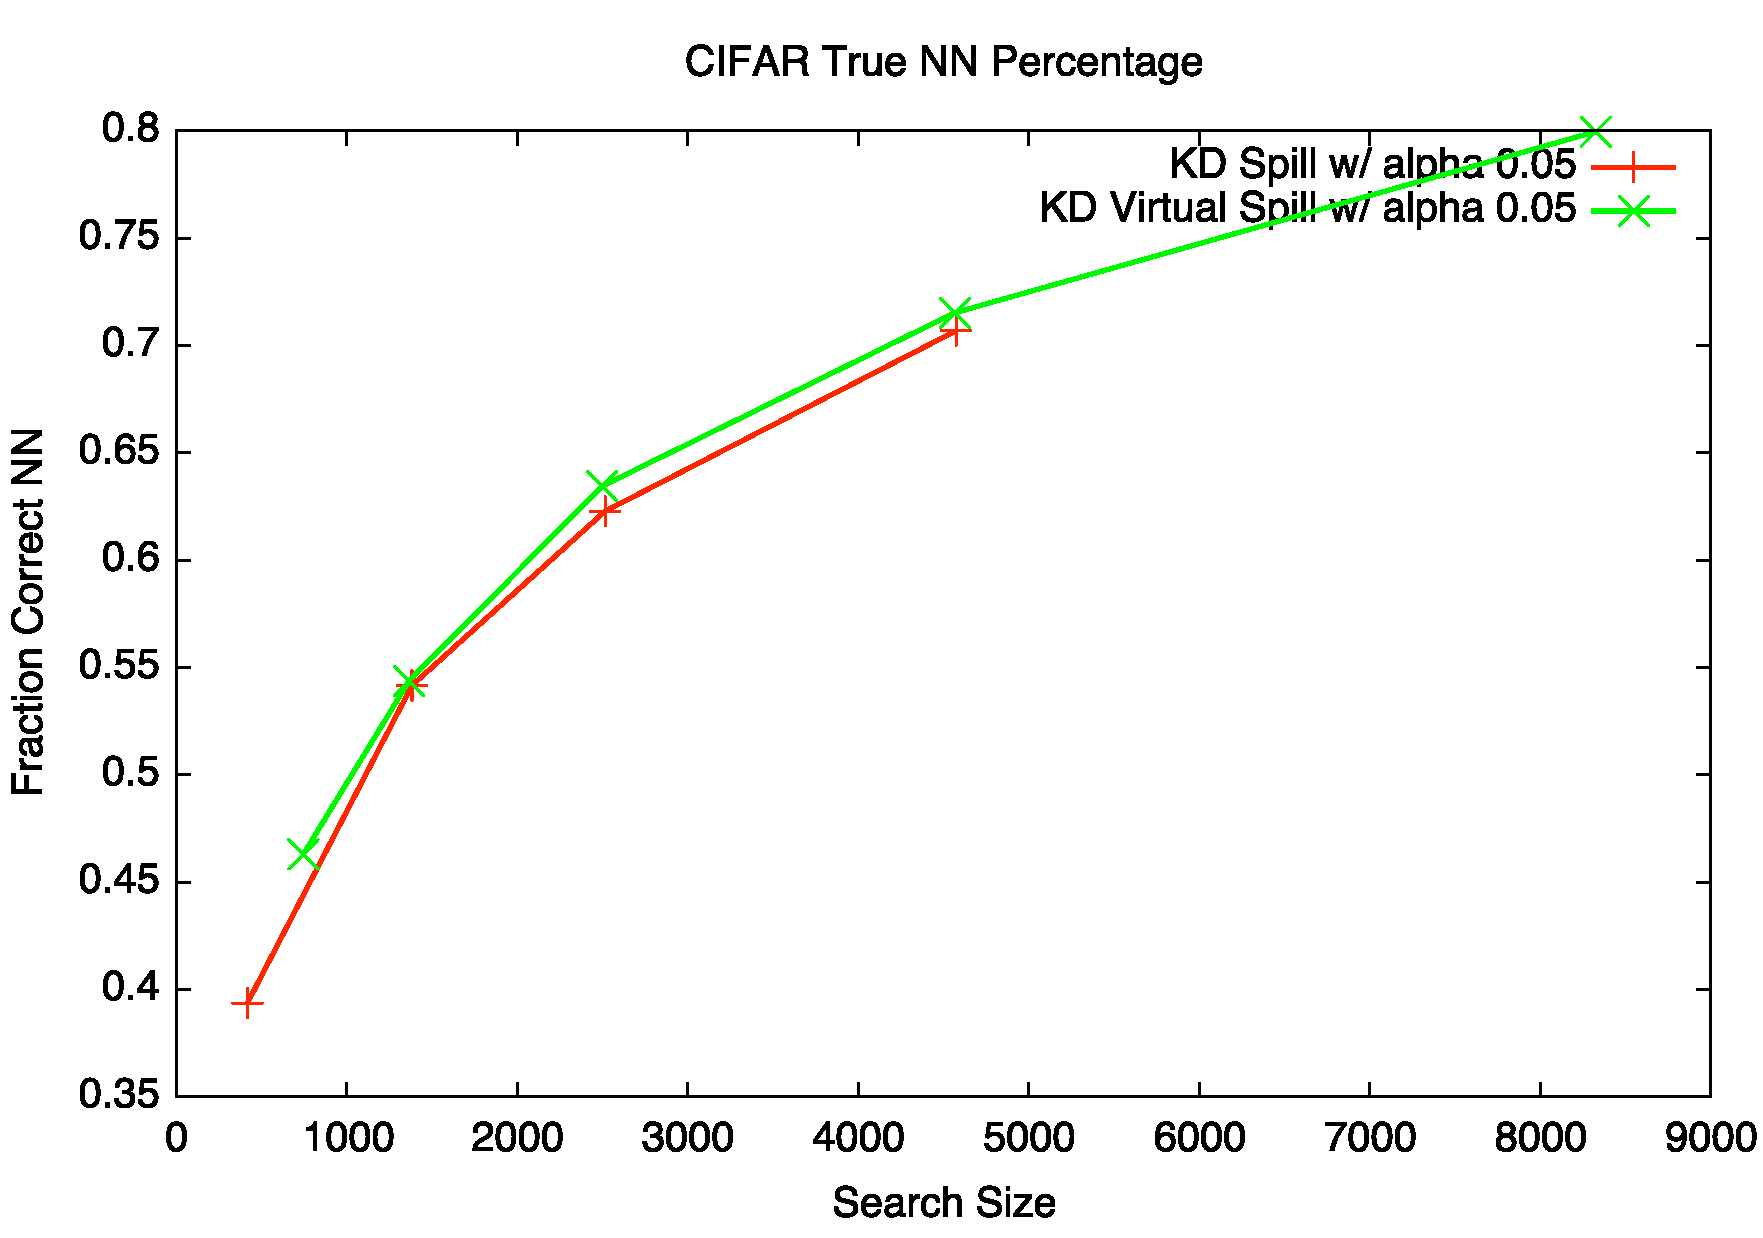
\includegraphics[width=.5\textwidth]{kd_vspill_vs_kd_spill_point05.pdf} \\
   \end{tabular}
\end{figure}

\section{Conclusion}








\end{document}